Испытания на воздействие пониженной температуры среды по \\ \ref{t_k_m} настоящих~ТУ проводят следующим образом:
%
\begin{enumerate}
	\item собирают схему в соответствии с рисунком \ref{fig:preheat} и прогревают \dut \ с помощью внутренней системы прогрева в течение не менее~$0,5$~ч;
	\item \dut \ помещают в камеру холода, в которой температура заранее доведена до рабочей пониженной температуры, указанной в \ref{t_k_m} настоящих~ТУ; 
	\item собирают схему проверки в соответствии с рисунком~\ref{fig:capacity_camera} в течение не более $5$ минут;
%
		\begin{figure}[!htb]
			\centering
			\includegraphics[page=4]{schema}
			\begin{picdescription}
				\item \ESKDtheTitle \ \RN;
			\end{picdescription}
			\begin{picdescription}[label={E\arabic* ---}, ref={E\arabic*}, before={\vspace{0pt}\small}]
				\item\label{d:preheat} \hyperref[e:preheat]{Жгут \preheatRN}.
			\end{picdescription}
			\caption{Схема прогрева \dut \ }
			\label{fig:preheat}
		\end{figure}
%
	\item средства измерения подготавливают к работе согласно прилагаемым к ним инструкциям по эксплуатации;
	\item производят проверки по \treb \ настоящих~ТУ;
	\item отсоединяют жгут \ref{d:cable} от Стенда нагрузочного \ref{d:stend};
	\item в камере устанавливают предельную пониженную температуру, указанную в \ref{t_k_m} настоящих~ТУ;
	\item после установления заданного значения предельной температуры  \dut \ выдерживают в камере не менее $24$~ч;
	\item температуру в камере повышают до нормальной и, после выдержки в течение $2$~ч, производят проверки по \treb, \trebafter \ настоящих~ТУ.
\end{enumerate}

\dut \ считается выдержавшим проверку по \ref{t_k_m} настоящих~ТУ, если \dut \ соответствует требованиям \treb \ настоящих~ТУ в процессе испытания и соответствует \trebafter \ настоящих~ТУ после испытания.